\documentclass[tikz, border=1pt]{standalone}

\usepackage{xcolor}
\usetikzlibrary{arrows.meta,decorations.pathreplacing,angles,quotes}

\begin{document}
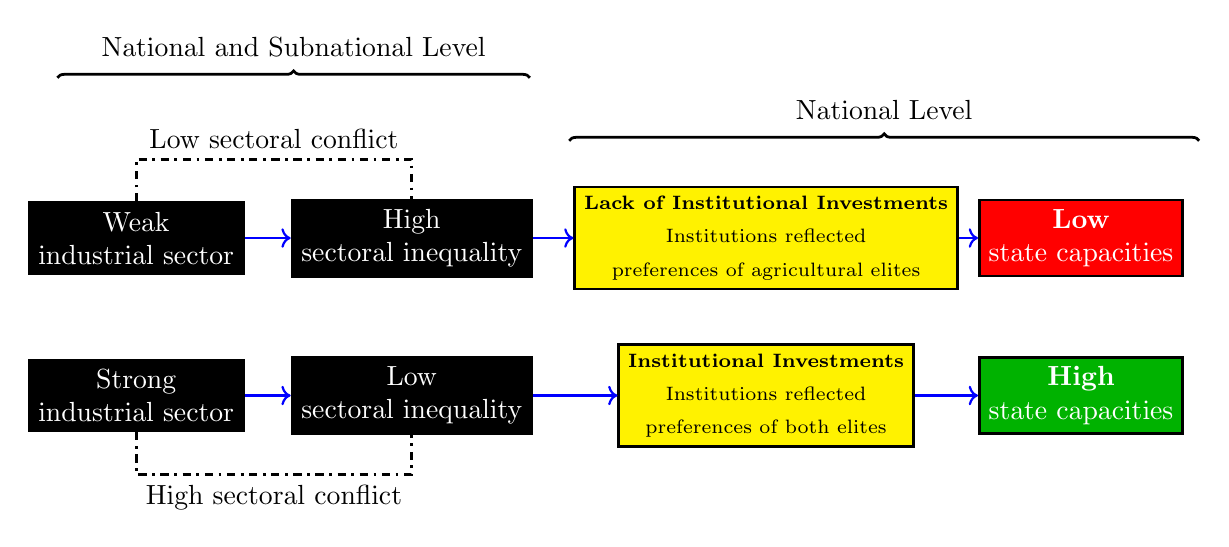
\begin{tikzpicture}[line width=1pt]


\draw[decoration={brace,raise=1pt},decorate]
  (0,4) -- node[above=5pt] {National and Subnational Level} (6,4);

\draw[decoration={brace,raise=1pt},decorate]
  (6.5,3.2) -- node[above=5pt] {National Level} (14.5,3.2);


% 1
\node[draw,align=center,fill=black,text=white] (ArgumentA1) at (1,0) {Strong\\industrial sector};
\node[draw,align=center,fill=black,text=white] (ArgumentB1) at (4.5,0) {Low\\sectoral inequality};

\node[draw,align=center,fill=yellow,text=black] (ArgumentD1) at (9,0) {{\scriptsize {\bf Institutional Investments}}\\{\scriptsize Institutions reflected}\\ {\scriptsize preferences of both elites}};

% 1
\node[draw,fill=black!30!green,text=white,align=center] (ArgumentA3) at (13,0) {{\bf High}\\ state capacities};



\draw[->,draw=blue,thick] (ArgumentD1) to (ArgumentA3);
\draw[->,draw=blue,thick] (ArgumentA1) to (ArgumentB1);
\draw[->,draw=blue,thick] (ArgumentB1) to (ArgumentD1);


\draw[dash dot] (ArgumentA1) -- ++(0,-1) -| (ArgumentB1) node[below, near start] {High sectoral conflict};

 

\node at (6., -1.0) {};



% 2
\node[draw,align=center,fill=black,text=white] (ArgumentA2) at (1,2) {Weak\\industrial sector};
\node[draw,align=center,fill=black,text=white] (ArgumentB2) at (4.5,2) {High\\sectoral inequality};
\node[draw,,align=center,fill=yellow,text=black] (ArgumentD2) at (9,2) {{\scriptsize {\bf Lack of Institutional Investments}}\\{\scriptsize Institutions reflected}\\ {\scriptsize preferences of agricultural elites}};



\node[draw,fill=red,text=white,align=center] (ArgumentA4) at (13,2) {{\bf Low}\\state capacities};


\draw[->,draw=blue,thick] (ArgumentD2) to (ArgumentA4);
\draw[->,draw=blue,thick] (ArgumentA2) to (ArgumentB2);
\draw[->,draw=blue,thick] (ArgumentB2) to (ArgumentD2);



\draw[dash dot] (ArgumentA2) -- ++(0,1) -| (ArgumentB2)
node[above, near start] {Low sectoral conflict};




\node at (6., -1.0) {};












  
\end{tikzpicture}
\end{document}